\begin{table}
\centering
\begin{tabular}{ll}
Feature                          & Data Type              \\ \hline
Gender                           & Categorical            \\
Age                              & Numerical (discrete)   \\
WBC (White blood cell count)     & Numerical (continuous) \\
Platelets                        & Numerical (continuous) \\
Neutrophils                      & Numerical (continuous) \\
Lymphocytes                      & Numerical (continuous) \\
Monocytes                        & Numerical (continuous) \\
Eosinophils                      & Numerical (continuous) \\
Basophils                        & Numerical (continuous) \\
CRP (C-reactive protein)         & Numerical (continuous) \\
AST (aspartate aminotransferase) & Numerical (continuous) \\
ALT (alanine aminotransferase)   & Numerical (continuous) \\
ALP (alkaline phosphatase)       & Numerical (continuous) \\
GGT (gamma glutamyl transferase) & Numerical (continuous) \\
LDH (lactate dehydrogenase)      & Numerical (continuous) \\
SWAB                             & Categorical           
\end{tabular}
\caption{Overview over all features of the data set}
\label{tab:overview-features}
\end{table}
\begin{table}
\centering
\begin{tabular}{lllll}
Feature                          & Unit                    & Mean   & Std    & 
Median \\ \hline
Age                              & Years                   & 61.33  & 18.05  & 
64     \\
White Blood Cell Count (WBC)     & $10^9$/L & 8.49   & 4.89   & 
7.10   \\
Platelets                        & $10^9$/L & 224.91  & 102.61  & 
204.00 \\
Neutrophils                      & $10^9$/L & 4.64   & 4.50   & 
3.90   \\
Lymphocytes                      & $10^9$/L & 0.88   & 0.87   & 
0.80   \\
Monocytes                        & $10^9$/L & 0.45   & 0.44   & 
0.40   \\
Eosinophils                      & $10^9$/L & 0.04   & 0.12   & 
0.00   \\
Basophils                        & $10^9$/L & 0.01   & 0.03   & 
0.00   \\
C-reactive protein (CRP)         & mg/L                    & 88.93  & 94.32  & 
53.10  \\
Aspartate Aminotransferase (AST) & U/L                     & 53.81  & 57.59  & 
36.00  \\
Alanine Aminotransferase (ALT)   & U/L                     & 42.82  & 45.43  & 
30.00  \\
Alkaline Phosphatase (ALP)       & U/L                     & 42.21  & 75.71  & 
68.00  \\
Gamma Glutamyl Transferase (GGT) & U/L                     & 40.20  & 101.29 & 
0.00  \\
Lactate dehydrogenase (LDH)      & U/L                     & 264.54 & 238.53 
& 254.00
\end{tabular}
\caption{Descriptive statistics for numerical features in data set (including 
missing values as in \cite{RN127})}
\label{tab:feature-dist-NAN}
\end{table}
\begin{table}
\centering
\begin{tabular}{ll}
Feature                          & Number of NaN (in \%) \\ \hline
Gender                           & 0 (0 \%)              \\
Age                              & 2 (0.72 \%)           \\
WBC (White blood cell count)     & 2 (0.72 \%)           \\
Platelets                        & 2 (0.72 \%)           \\
Neutrophils                      & 70 (25.09 \%)         \\
Lymphocytes                      & 71 (25.45 \%)         \\
Monocytes                        & 70 (25.09 \%)         \\
Eosinophils                      & 70 (25.09 \%)         \\
Basophils                        & 71 (25.45 \%)         \\
CRP (C-reactive protein)         & 6 (2.15 \%)           \\
AST (aspartate aminotransferase) & 2 (0.72 \%)           \\
ALT (alanine aminotransferase)   & 13 (4.66 \%)          \\
ALP (alkaline phosphatase)       & 148 (53.05 \%)        \\
GGT (gamma glutamyl transferase) & 143 (51.25 \%)        \\
LDH (lactate dehydrogenase)      & 85 (30.47 \%)         \\
SWAB                             & 0 (0 \%)             
\end{tabular}
\caption{Number of missing values and their proportion the total number of data 
points}
\label{tab:nan-overview}
\end{table}
\begin{table}[ht]
\centering
\begin{tabular}{lllll}
Feature                          & Unit                    & Mean   & Std    & 
Median \\ \hline
Age                              & Years                   & 61.78  & 17.81  & 
64     \\
White Blood Cell Count (WBC)     & $10^9$/L & 8.55   & 4.86   & 
7.10   \\
Platelets                        & $10^9$/L & 226.5  & 101.2  & 
205.00 \\
Neutrophils                      & $10^9$/L & 6.20   & 4.17   & 
5.10   \\
Lymphocytes                      & $10^9$/L & 1.19   & 0.80   & 
1.00   \\
Monocytes                        & $10^9$/L & 0.61   & 0.41   & 
0.50   \\
Eosinophils                      & $10^9$/L & 0.06   & 0.13   & 
0.00   \\
Basophils                        & $10^9$/L & 0.01   & 0.04   & 
0.00   \\
C-reactive protein (CRP)         & mg/L                    & 90.89  & 94.42  & 
54.20  \\
Aspartate Aminotransferase (AST) & U/L                     & 54.20  & 57.61  & 
36.00  \\
Alanine Aminotransferase (ALT)   & U/L                     & 44.92  & 45.50  & 
31.00  \\
Alkaline Phosphatase (ALP)       & U/L                     & 89.89  & 89.09  & 
71.00  \\
Gamma Glutamyl Transferase (GGT) & U/L                     & 82.48  & 132.70 & 
41.00  \\
Lactate dehydrogenase (LDH)      & U/L                     & 380.45 & 193.98 & 
328.00
\end{tabular}
\caption{Descriptive statistics for numerical features in data set (excluding 
missing values)}
\label{tab:feature-dist}
\end{table}
% non-normality of data with graphs from python as visualization aid
\begin{figure}[ht]
    \centering
    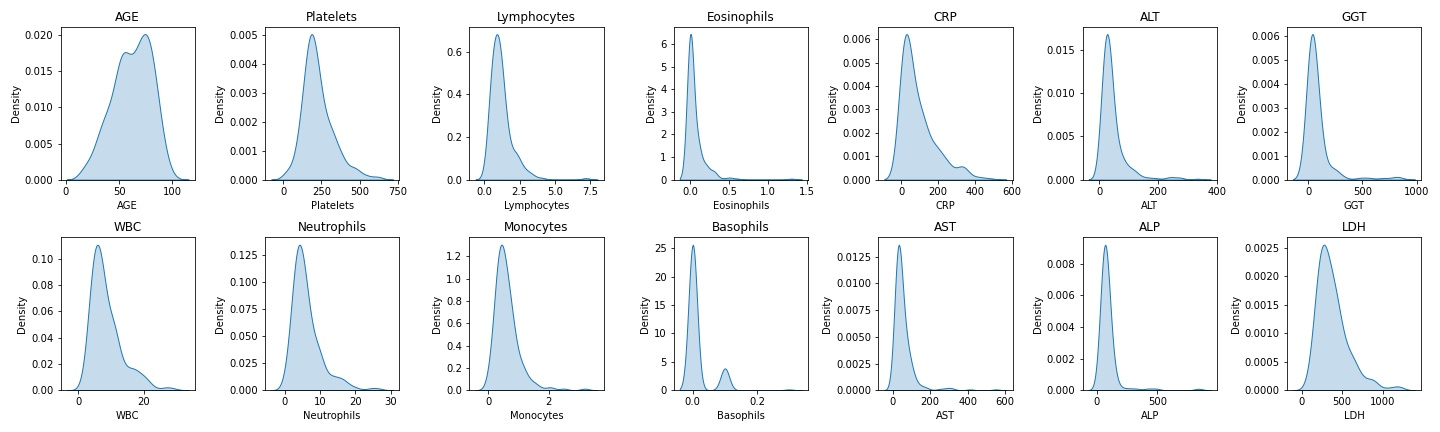
\includegraphics[width=1.1\textwidth]{figures/density_no_split.jpg}
    \caption{Kernel density plots of the numerical features of the data set}
    \label{fig:density}
\end{figure}

\begin{table}
\begin{tabular}{lll}
Feature                          & Test statistic & p-value \\ \hline
Age                              & 0.976          & 0.000   \\
WBC (White blood cell count)     & 0.873          & 0.000   \\
Platelets                        & 0.930          & 0.000   \\
Neutrophils                      & 0.838          & 0.000   \\
Lymphocytes                      & 0.785          & 0.000   \\
Monocytes                        & 0.811          & 0.000   \\
Eosinophils                      & 0.457          & 0.000   \\
Basophils                        & 0.395          & 0.000   \\
CRP (C-reactive protein)         & 0.836          & 0.000   \\
AST (aspartate aminotransferase) & 0.556          & 0.000   \\
ALT (alanine aminotransferase)   & 0.629          & 0.000   \\
ALP (alkaline phosphatase)       & 0.420          & 0.000   \\
GGT (gamma glutamyl transferase) & 0.500          & 0.000   \\
LDH (lactate dehydrogenase)      & 0.877          & 0.000  
\end{tabular}
\caption{Results of Shapiro-Wilk test for normality for numerical features of 
the data set}
\label{tab:shapiro-wilk}
\end{table}
